\documentclass[10pt,letterpaper]{article}
\usepackage[margin=0.55in]{geometry}
\usepackage{amsmath,graphicx,booktabs,caption}
\captionsetup{font=footnotesize,labelfont=bf,skip=3pt}
\pagestyle{empty}
\begin{document}
\begin{center}{\large\bfseries Your universe at the best fit: thick ordinary-matter shell plus a CoE core (relativistic fit)}\end{center}
\vspace{-8pt}
\begin{figure}[h]\centering
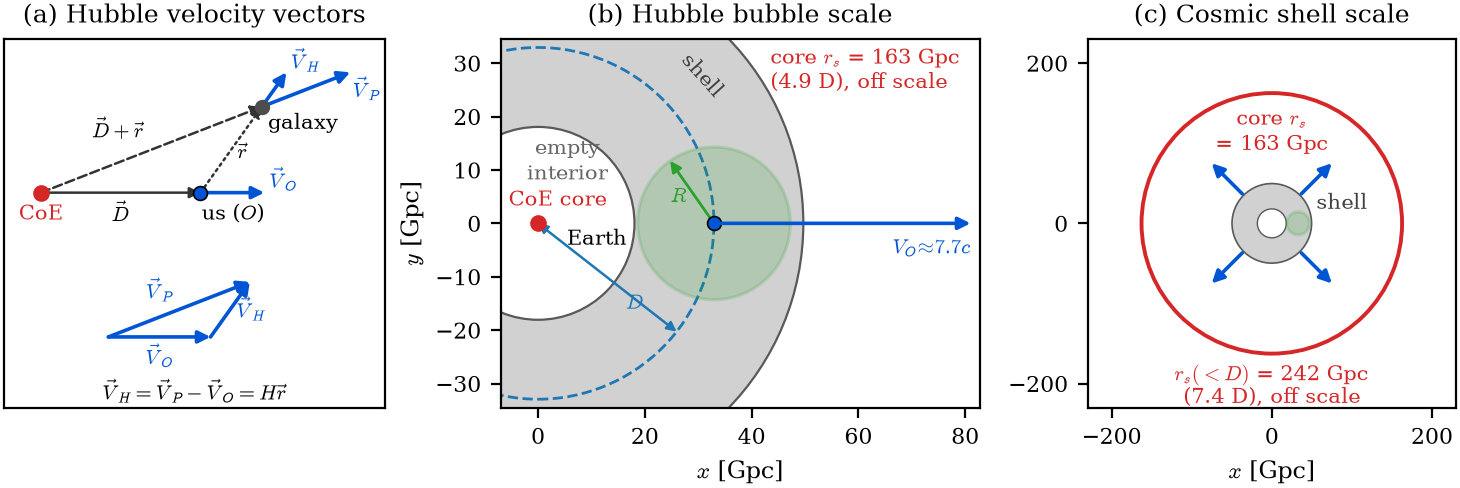
\includegraphics[width=\textwidth]{universe_thin_drawing.png}
\caption{Three scales at the relativistic best fit; (b) and (c) are to scale in Gpc. (a) Hubble velocity vectors. In a Sedov--Taylor blast wave (Taylor 1950; Sedov 1959) $\vec V = k\,\times$(position from the CoE), so we move with $\vec V_O = k\vec D$ and a galaxy with $\vec V_P = k(\vec D+\vec r)$; then $\vec V_P-\vec V_O = k\vec r$ is Hubble's law, so $k = H$ and the CoE drops out. (b) Hubble bubble: ordinary-matter shell (grey, $\Omega_s=0.049$) from $R_{\rm in}=18.1$ to $R_{\rm out}=49.7$~Gpc around an empty interior and the CoE core; dashed circle $D=32.9$~Gpc through Earth; green vision sphere $R=14.3$~Gpc; Earth moves along $+x$ (anti-CoE, $\ell_0=13.5^\circ$) at $V_O=H_0D/c\approx7.7\,c$. (c) Cosmic shell: the core's Schwarzschild radius $r_s=163$~Gpc ($4.9\,D$); $r_s$ of all mass inside $D$ is 242~Gpc ($7.4\,D$), off scale. Blue arrows are velocities. The fit is exact relativistic (LTB), with ordinary matter only.}
\end{figure}
\vspace{-10pt}
\noindent\begin{minipage}[t]{0.40\textwidth}\vspace{0pt}\centering
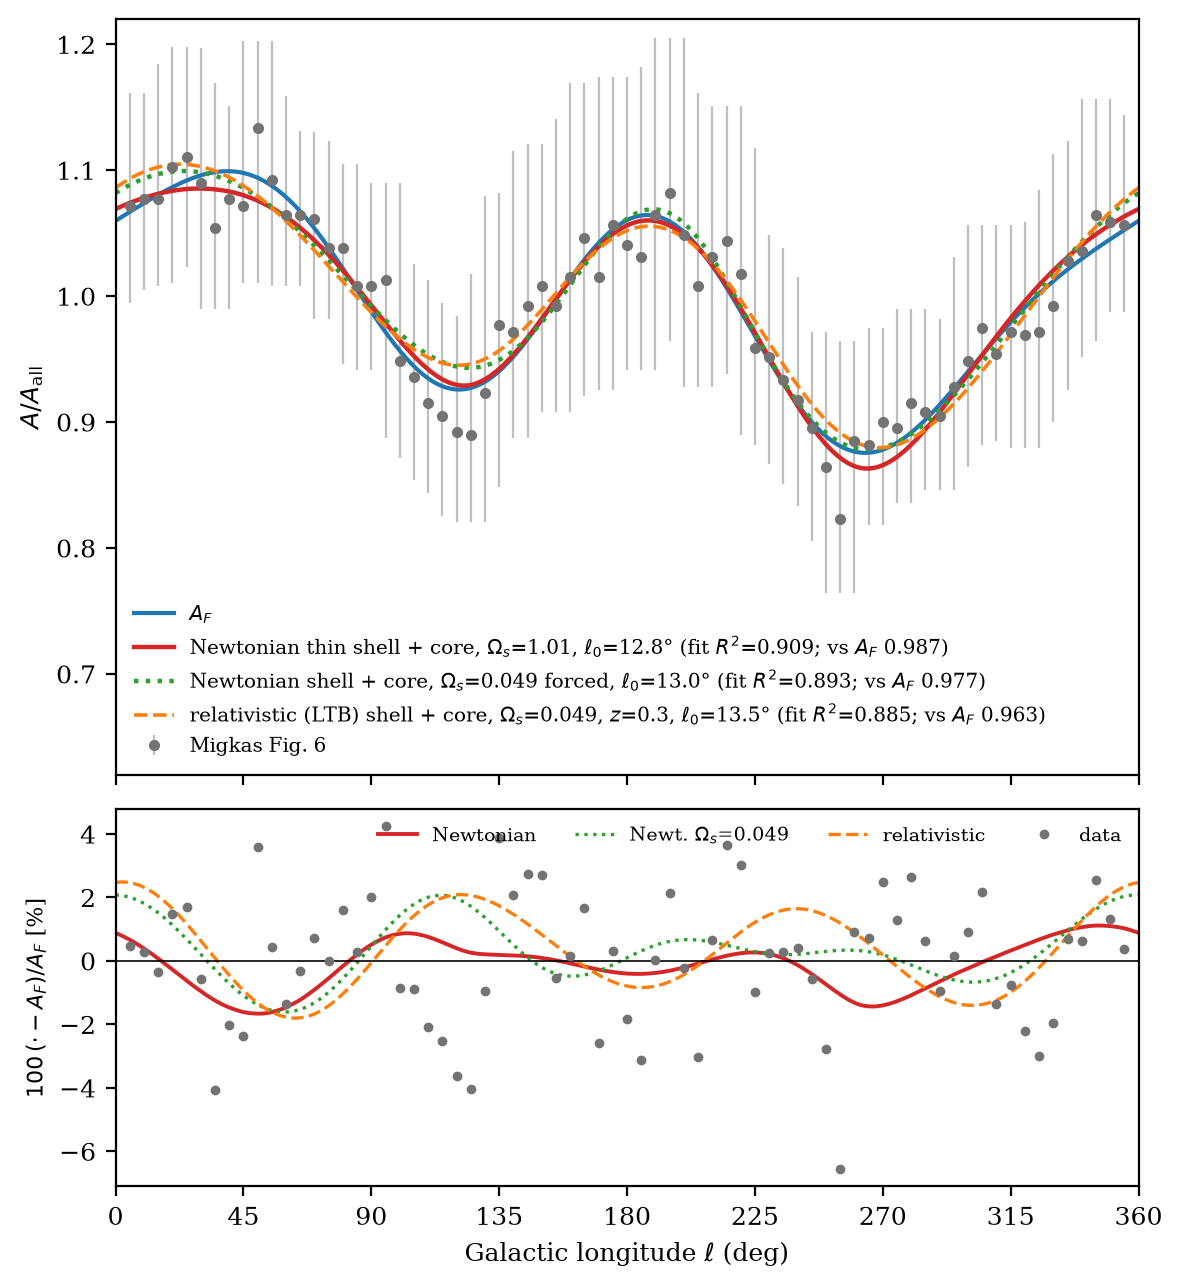
\includegraphics[width=\textwidth]{universe_thin_Achart.png}
\captionof{figure}{Migkas points with error bars, $A_F$ and model A, normalised to the sky mean. Solid red: Newtonian thin shell with core ($\Omega_s=1.01$, $R^2=0.909$). Dotted green: Newtonian with $\Omega_s=0.049$ forced, $R^2=0.893$ (0.54 geometry only). Dashed orange: relativistic (LTB) ordinary-matter shell with core ($\Omega_s=0.049$, all parameters free), sampled at the Migkas cluster distance ($z=0.3$, 1.19~Gpc), $R^2=0.885$ (0.57 without the sine). Lower panel: percent differences from $A_F$.}
\end{minipage}\hfill
\begin{minipage}[t]{0.59\textwidth}\vspace{0pt}\centering\scriptsize\setlength{\tabcolsep}{1.5pt}\renewcommand{\arraystretch}{0.93}
\captionof{table}{Best-fit values in your sheet's cells. Newtonian: integrated model ($G$ real, from $0.01\,t_0$, fixed in space, $H_0=70$), thin shell $D-R$ to $D+R$. Newtonian $\Omega_s$=0.049: same model with the shell density forced to ordinary matter. Relativistic: exact LTB, ordinary-matter shell; $D$, $M_c$, $R_{\rm in}$, $R_{\rm out}$, $\ell_0$, Amp, $\varphi$ all free (shell $\ge R$ each side of Earth); $H=78$/66 km\,s$^{-1}$\,Mpc$^{-1}$ along/across the axis. $R^2$ in brackets: geometry only (no sine). B27 is all mass inside $D$.}
\begin{tabular}{lllll}\toprule
Cell & Quantity & \begin{tabular}[b]{@{}l@{}}Newtonian,\\ $\Omega_s$ free\end{tabular} & \begin{tabular}[b]{@{}l@{}}Newtonian,\\ $\Omega_s$=0.049\end{tabular} & \begin{tabular}[b]{@{}l@{}}Relativistic,\\ $\Omega_s$=0.049,\\ $M_c$ free\end{tabular}\\\midrule
C23 & $D/R$ & 6.554 & 3.439 & 2.303\\
D23 & $L_c/D$ (core size) & 0.0050 (bound) & 0.0050 & 0.0050\\
B29 & $R$ & $4.4127\times10^{23}$ km & same & same\\
 &  & (14.30 Gpc) &  & \\
B28 & $D$ & $2.8919\times10^{24}$ km & $1.5174\times10^{24}$ km & $1.0164\times10^{24}$ km\\
 &  & (93.72 Gpc) & (49.17 Gpc) & (32.94 Gpc)\\
B30 & $L_c$ & $1.45\times10^{22}$ km & $7.59\times10^{21}$ km & $5.08\times10^{21}$ km\\
 &  & (0.469 Gpc) & (0.246 Gpc) & (0.165 Gpc)\\
B27 & $M(<D)$, total & $3.72\times10^{56}$ kg & $4.56\times10^{54}$ kg & $5.04\times10^{54}$ kg\\
 &  & $1.87\times10^{26}$ $M_\odot$ & $2.29\times10^{24}$ $M_\odot$ & $2.53\times10^{24}$ $M_\odot$\\
 & $M_c$, core & $2.47\times10^{54}$ kg & $2.31\times10^{53}$ kg & $3.38\times10^{54}$ kg\\
 &  & $1.24\times10^{24}$ $M_\odot$ & $1.16\times10^{23}$ $M_\odot$ & $1.70\times10^{24}$ $M_\odot$\\
 & $M_c/M_{\rm crit}(D)$ & 0.00265 & 0.00171 & 0.083\\
 & $M_{\rm shell}(<D)$ & $3.70\times10^{56}$ kg & $4.33\times10^{54}$ kg & $1.66\times10^{54}$ kg\\
 & $M_{\rm shell}$, total & $8.71\times10^{56}$ kg & $1.70\times10^{55}$ kg & $6.48\times10^{54}$ kg\\
 & $M$ within $R$ & $3.35\times10^{54}$ kg & $1.62\times10^{53}$ kg & $1.62\times10^{53}$ kg\\
 & $M_{\rm hole}$ & $5.74\times10^{56}$ kg & $2.28\times10^{54}$ kg & $3.27\times10^{53}$ kg\\
BA57 & Amp & $-$0.1240 & $-$0.0622 & $-$0.0558\\
BA59 & $\varphi$ & 1.264 rad & 0.929 rad & 0.848 rad\\
 & $\ell_0$ & 12.82$^\circ$ & 13.0$^\circ$ & 13.5$^\circ$\\
\midrule
 & $\Omega_s$ & 1.012 & 0.049 & 0.049\\
 & $\rho_s$ & $9.32\times10^{-27}$ kg\,m$^{-3}$ & $4.51\times10^{-28}$ kg\,m$^{-3}$ & $4.51\times10^{-28}$ kg\,m$^{-3}$\\
 & $R_{\rm in}$ & 79.4 Gpc ($D-R$) & 34.5 Gpc & 18.1 Gpc\\
 & $R_{\rm out}$ & 108.0 Gpc ($D+R$) & 70.3 Gpc & 49.7 Gpc\\
 & $r_s$, core & 119 Gpc (1.27\,$D$) & 11 Gpc (0.2\,$D$) & 163 Gpc (4.9\,$D$)\\
 & $r_s$, all mass $<D$ & 17{,}907 Gpc (191\,$D$) & 219 Gpc (4.5\,$D$) & 242 Gpc (7.4\,$D$)\\
\midrule
 & $(V_O/v_{\rm esc})^2$ / $2E/c^2$ & 0.901 (bound) & 8.0 (unbound) & +45 (unbound)\\
 & Turnaround radius & 991 Gpc (10.6\,$D$) & none & none\\
 & Age $t_0$ & 13.8 Gyr & 13.9 Gyr & 13.0 Gyr\\
 & $\delta$ across sphere & 0 & 0 & 0\\
 & fit $R^2$ vs Migkas & 0.909 & 0.893 (0.54) & 0.885 (0.57)\\
 & fit $R^2$ vs $A_F$ & 0.987 & 0.977 & 0.963\\
\bottomrule
\end{tabular}
\end{minipage}
\par\vspace{6pt}\noindent{\scriptsize\textbf{References.} Taylor, G.~I. 1950, Proc.\ R.\ Soc.\ Lond.\ A, 201, 159. Sedov, L.~I. 1959, Similarity and Dimensional Methods in Mechanics (New York: Academic Press).\par}
\end{document}
